\documentclass[11pt, a4paper]{article}
\usepackage{rminterim}
\begin{document}

% Your project title etc goes here
\title{\textbf{\textsc{\Huge My Project Title}}\\ 
        {\Large Milestone Report for Research Project Module 5E1}
      }
\author{Oscar Cat \\ 
        Trinity College Dublin \\
        {\tt oscar.cat@tcd.ie}
        }
%\address{Probably not needed}

\date{May 2021}

\maketitle

% This just shows you how to make a manually reformatted section within a page .. which functions like an independent page.
% Its really useful if you want to highlight something and you can even box it up with \fbox 
% You will need this declaration at the start of your report.
\begin{center}
\fbox{\begin{minipage}[t]{0.8\linewidth}
\textit{
This report is submitted in part fulfilment for the assessment required in 5E1 Research Project.  I have read and I understand the plagiarism provisions in the General Regulations of the University Calendar for the current year. These are found in Parts II and III at \myhref{http://www.tcd.ie/calendar}{ http://www.tcd.ie/calendar}.}
\end{minipage}}
\end{center}

% You might not want an abstract so this is up to you
% Just comment it out and use it.
%\begin{abstract}
%An abstract might go here if necessary. An abstract might go here if necessary. An abstract might go here if necessary. An abstract might go here if necessary. An abstract might go here if necessary. An abstract might go here if necessary.
%\end{abstract}

This template is meant to be read as a an example of what your milestone report should looks like. In this preamble bit here you might want to say something like this ...

This report documents progress and discusses achievements against the project plan submitted in Jan 2021. It outlines challenges and presents a plan for the remainder of the project. 

\section{A review of the Project Goals}
The principal goal of this project is to develop a new technique for modeling the weather patterns in a small area. This problem is important because Meterological reports cover entire counties at a scale of 100's of square kilometers but people are affected by weather patters on the scale of 100's of square metres. Personal weather forecasting is expected to become a major function of social media applications within the next ten years \cite{boykov_2001}. In the following we briefly state and explain any modification to the project goals.

{\noindent \bf A public implementation of the work of Boykov et al \cite{boykov_2001} : } This is the major piece of previous work which first presented the idea of personal weather forecasting. However we discovered that their work relied heavily on an implementation of Quantum flux prediction which is not available publicly. Therefore we altered the project goals to reflect this new piece of work required.

{\noindent \bf Design of a personal weather database: } This remains a key project goal and we have made progress toward this goal as discussed later in this report.

{\noindent \bf Design of a personal weather forecaster: } We will not be able to create a full system app for a mobile phone as originally planned. Instead the final project outcome will be an algorithm for personal weather forecasting which can ingest examples from the database and then output a prediction for weather patterns for that individual over the next day on an hour by hour basis. The algorithm is being implemented in Matlab and the output is a .csv file.

\section{Updates to previous work}

The design of person-scale weather forecasting algorithms has been ongoing for at least 20 years \cite{dirac, xu_2013,haskell_1976}. In the interim report a brief outline of this work was presented. Since that time, we have become aware of other publications which affected the project plan. In particular, while in the interim report we mentioned that the work of Puri et al \cite{PURI199339} was the most relevant to our work we have since discovered that Yilin's work \cite{liyin_2010} is more relevant. 

In the work by Yilin an algorithm was presented for forecasting rainfall for a single field of corn in the USA. That field was 10 hectares in area. This is quite similar to our goal. Their algorithm works by \ldots.
Figure~\ref{equationofmarking} shows a block diagram of that system. 
\begin{figure}
  \begin{center}
  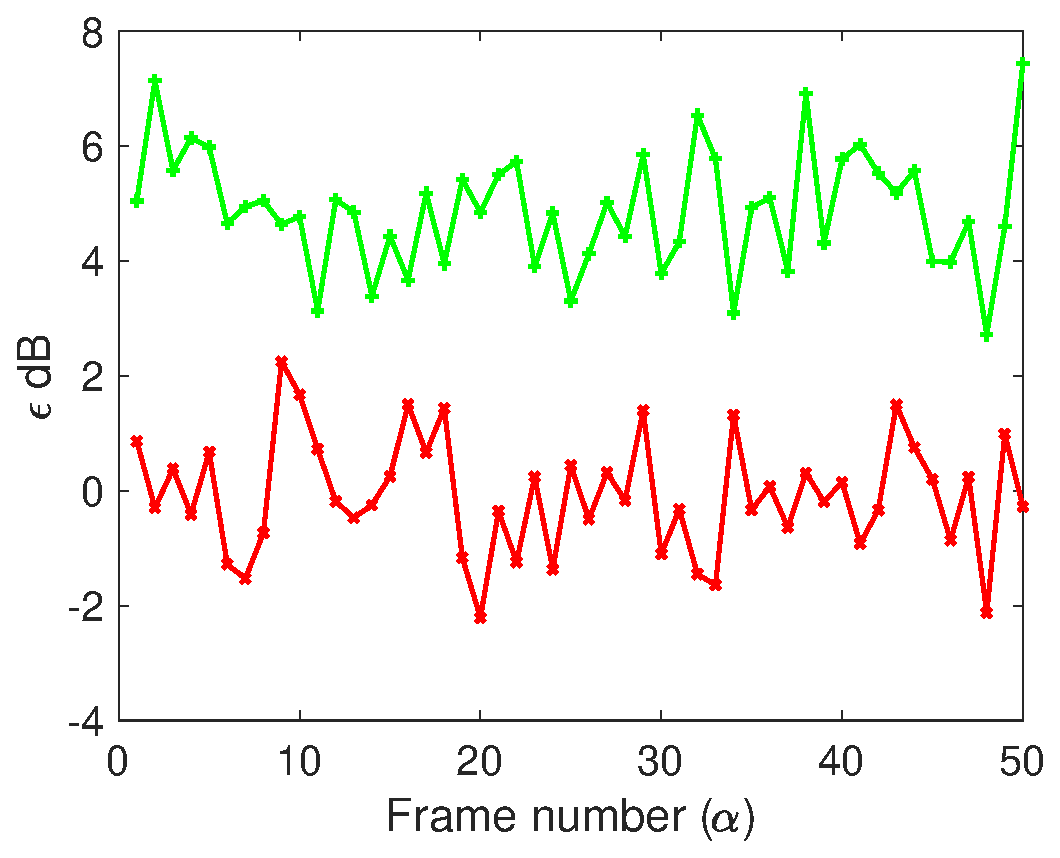
\includegraphics[width=0.7\linewidth]{alineplot.eps}
  \end{center}
  \caption{The distribution of mean squared errors from a difference as in equation~\ref{equationofmarking}. \label{bars}}
  \caprule %\noindent\rule{\linewidth}{0.5pt}
  \end{figure}
Having become aware of this work we have adjusted our design as presented in the milestones section.
The key equation is as follows.
\begin{equation}
    x_1 = \sum_{n=-4}^{N-1} \theta_n + 2\pi x_n - \int_{t=-\infty}^{\infty} \epsilon(t) dt \label{equationofmarking}
\end{equation}
Where $x_1$ is the amount of rainfall on day 1 after the recordings are complete, $\theta_n$ is the humidity measurement over the previous $N +4$ days, $\epsilon(t)$ is temperature at time $t$.
Our work centers now on estimating appropriate values of $\theta$ since it has become clear that erroneous $\theta$ causes unstable prediction.


% An example of two figures side by side
\begin{figure}
\centering
\begin{minipage}{0.45\textwidth}
\centering 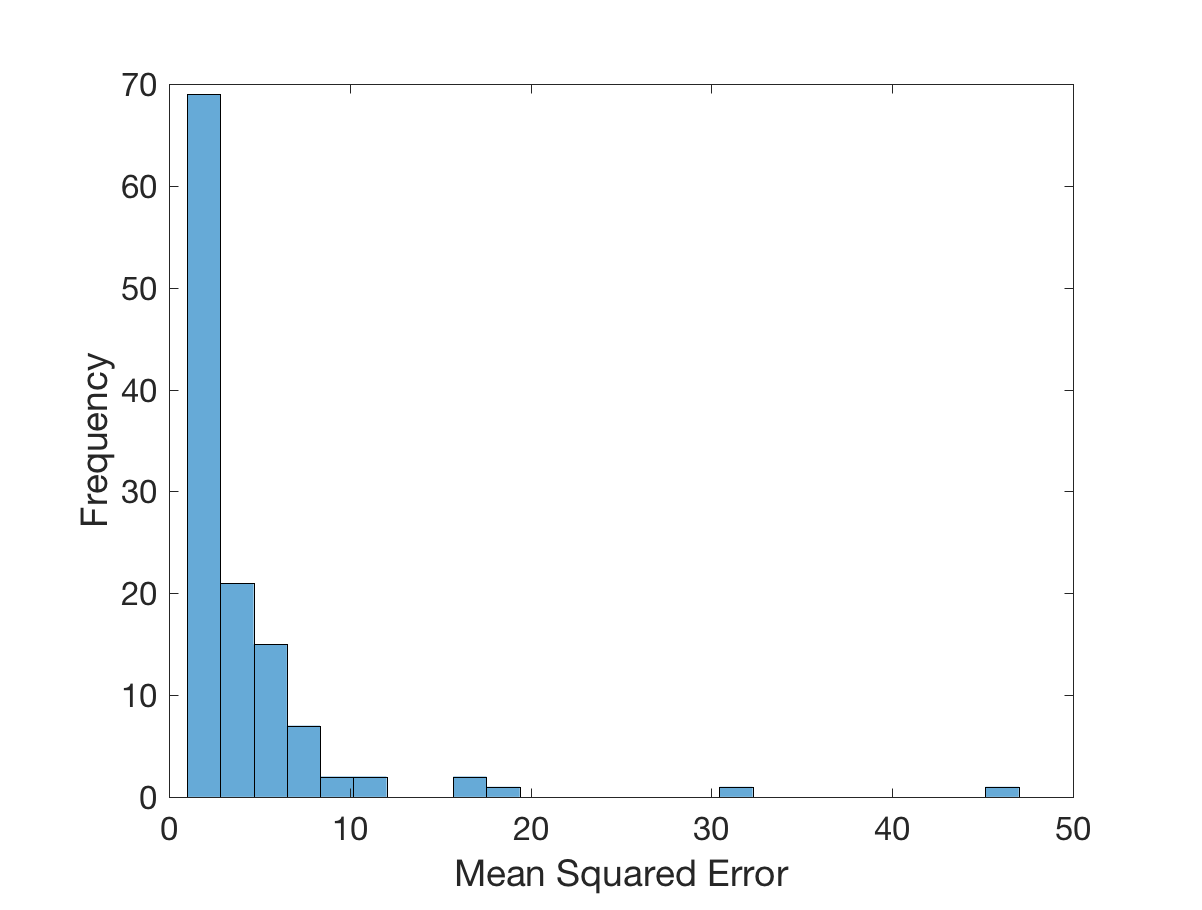
\includegraphics[width=\linewidth,]{bars.eps}
\end{minipage} \hspace*{0.25cm}
\begin{minipage}{0.45\textwidth}
\centering 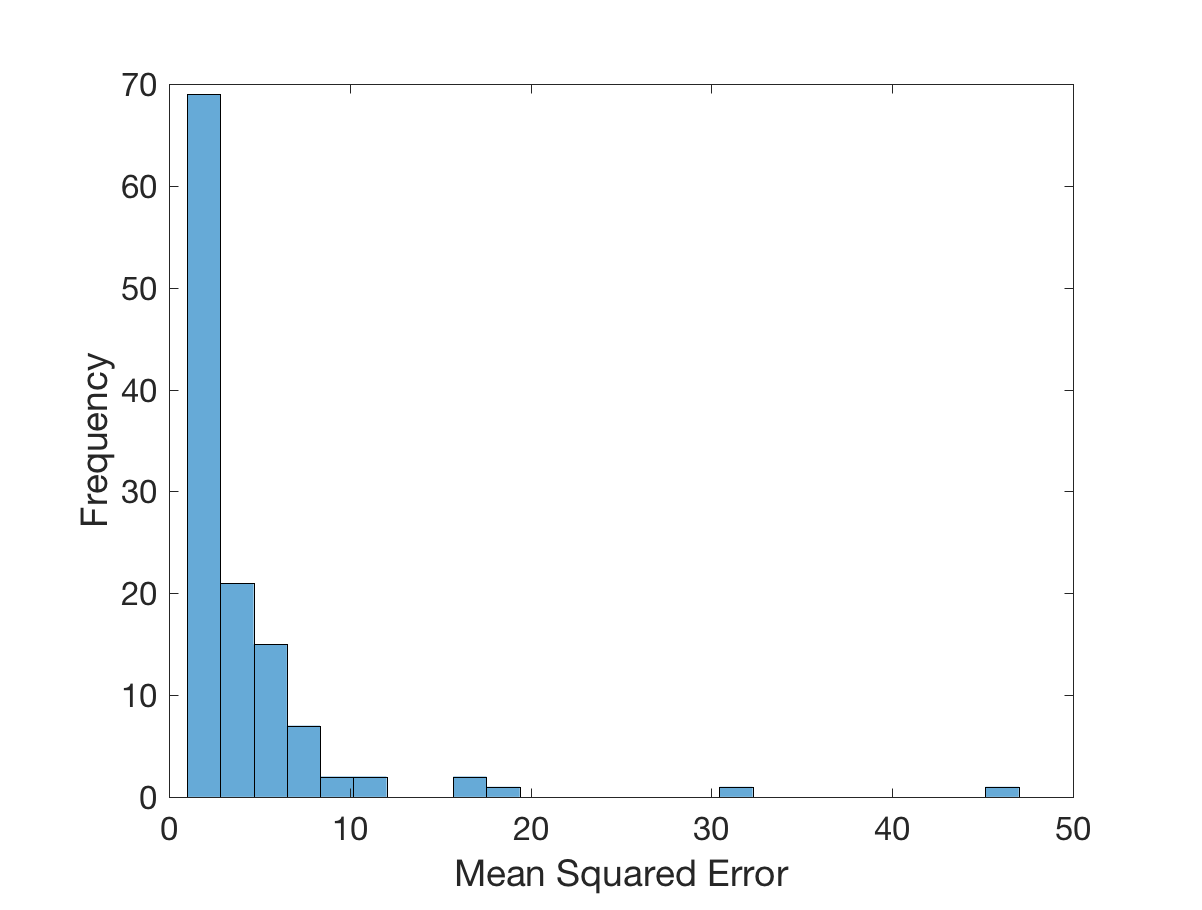
\includegraphics[width=\linewidth,]{bars.eps}
\end{minipage}
\caption{Left : Distribution of temperature measurements in the orbiting satellite. Right : Distribution of humidity in the spacecraft as a difference from target. \label{twofigs}}
\caprule
\end{figure}
\section{Milestone Review}

In the interim report, 4 milestones were set. These have been discussed with our supervisor at regular intervals and some alterations had to be made.  Each miestone is now discussed in turn.
\begin{itemize}
    \item {\bf M1 : Understanding Boykov \cite{boykov_2001}} This work relies heavily on Quantum Flux estimation and therefore we have had to devote some time to implementing and understanding Quantum Flux. The measurement of flux is important for predicting rainfall volumes on a local scale because of Heisenberg's principle. As described in \cite{linte_2016} the algorithm is based on measurements made with a spectroscope at two times per day. Spectral measurements of the ambient light in a field indicates how much water is held in the cloud cover overhead and that in turn is related to the possibility of rainfall. The algorithm is as follows\ldots
      \begin{enumerate}
        \item Wow
        \item Ipso Facto 
      \end{enumerate}
    This work was completed in February and then the paper by Boykov was critically assessed. The system was implemented as shown in Figure~\ref{twofigs}. We are currently generating results Preliminary findings indicate $\ldots$
    


    
    \item{\bf M2: Database creation}
       March was spent completing the databse work started in December. Through our collaboration with the Met Office and the use of an widely available consumer app we were able to collect 1 Million samples of subjective rainfall data from 500,000 citizens in Ireland. The data
       is shown as Figure~\ref{bars}. That shows $\ldots$
    \begin{figure}
  \begin{center}
  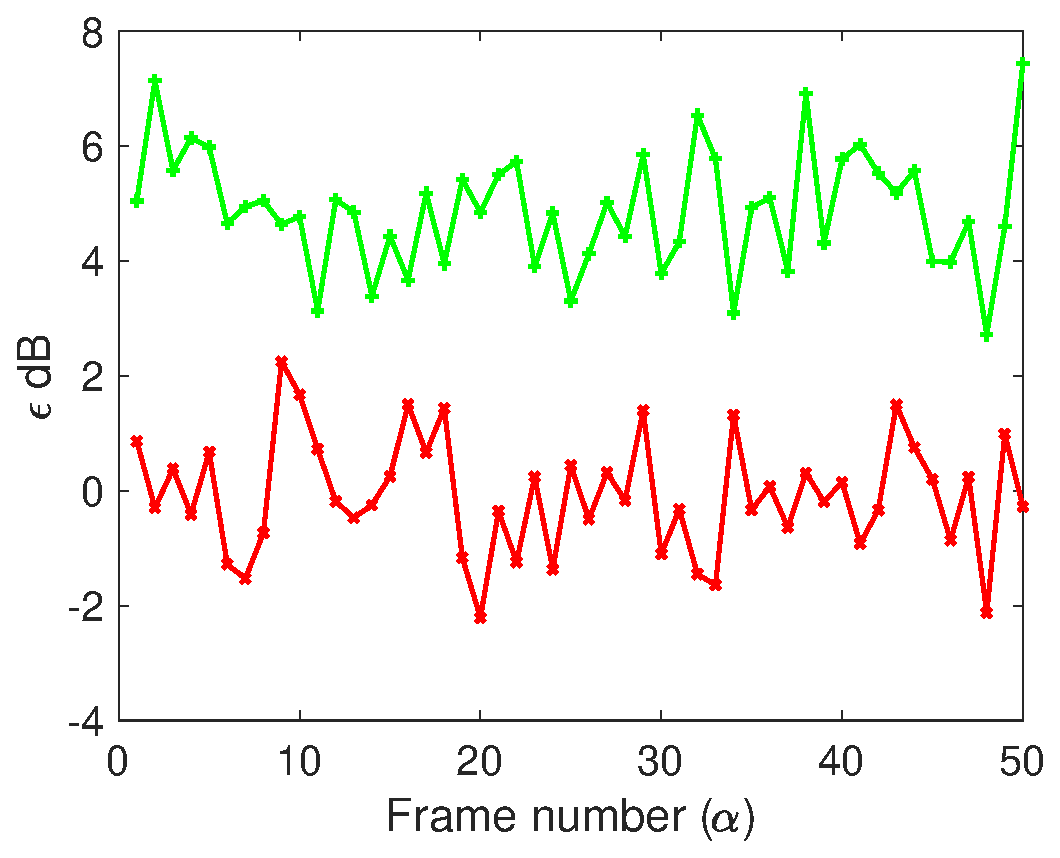
\includegraphics[width=0.7\linewidth]{alineplot.eps}
  \end{center}
  \caption{The distribution of subjective rainfall data. \label{bars}}
  \caprule %\noindent\rule{\linewidth}{0.5pt}
  \end{figure}
    
    \item{\bf M3: Rainfall Predictor 1}
    \item{\bf M4: Analysis of Results}

\end{itemize}

For the rest of the project the key milestones are as shown in the table below.
\begin{center}
\begin{tabular}{ccc} \hline
    Milestone & Date & Description \\ \hline 
    M1 & June 15th & Generate a prediction chart \\ \hline
    M2 & June 22nd & Complete implementation of algorithm \\ \hline
    M3 & June 30th & Outline draft of dissertation \\ \hline
    M3 & July 15th & First Draft of dissertation \\ \hline
    M4 & July 26th & Dissertation complete and submitted \\ \hline
\end{tabular}
\end{center}

\section{Final Comments}
The project has not proceeded exactly according to plan. This is because of the unanticipated difficulty in XXXX and YYYY. However we have largely mitigated these issues by doing ZZZ and HHH. Our results so far have shown that rainfall prediction is accurate to $\pm 1$ hour over the training data but not yet good enough for an application in the wild. Even if our final results remain at a low accuracy, we will still be in a position to write up our scientific journey so that others will learn from our experiences. Given the alterations to the project milestones as discussed We expect to be able to complete the dissertation on time.


% Here are my references
\bibliographystyle{acm}
\bibliography{myrefs}

\end{document}